% ============================================================
% Peared, საბაკალავრო პროექტის ანგარიში
% კომპილაცია: XeLaTeX (Overleaf-ზე: Menu -> Compiler -> XeLaTeX)
%
% ფონტი: გაიდის მიხედვით Sylfaen. თუ სისტემაზე Sylfaen არ დგას
% (მაგ. Overleaf-ზე), ატვირთეთ sylfaen.ttf პროექტში ან დროებით
% ჩაანაცვლეთ ქვემოთ fallback ფონტით (Noto Serif Georgian).
% ============================================================
\documentclass[12pt,a4paper]{article}

\usepackage{fontspec}
\IfFontExistsTF{Sylfaen}
  {\setmainfont{Sylfaen}}
  {\IfFontExistsTF{Noto Serif Georgian}
    {\setmainfont{Noto Serif Georgian}}
    {\setmainfont{DejaVu Serif}}}

\usepackage[a4paper,margin=1in]{geometry}
\usepackage{setspace}
\onehalfspacing
\usepackage{fancyhdr}
\usepackage{graphicx}
\usepackage{tikz}
\usetikzlibrary{positioning,arrows.meta,shapes.multipart,fit,calc,backgrounds}
\usepackage{newfloat}
\usepackage{caption}
\usepackage{booktabs}
\usepackage{enumitem}
\usepackage{titlesec}
\usepackage[hidelinks]{hyperref}

% ---------- ფერების პალიტრა დიაგრამებისთვის ----------
\definecolor{pcblue}{HTML}{2E6FB7}
\definecolor{pcblueL}{HTML}{DCEAF9}
\definecolor{pcgreen}{HTML}{2F8F5B}
\definecolor{pcgreenL}{HTML}{DFF3E7}
\definecolor{pcorange}{HTML}{D98A1F}
\definecolor{pcorangeL}{HTML}{FCEBD1}
\definecolor{pcred}{HTML}{C25B5B}
\definecolor{pcredL}{HTML}{F7DFDF}
\definecolor{pcpurple}{HTML}{7A5FA8}
\definecolor{pcpurpleL}{HTML}{EAE3F5}

% ---------- ცენტრირებული სათაურები ----------
\titleformat{\section}[block]{\centering\Large\bfseries}{}{0pt}{}
\titleformat{\subsection}[block]{\centering\large\bfseries}{}{0pt}{}

% ---------- ქართული სახელები სტანდარტული სათაურებისთვის ----------
\renewcommand{\contentsname}{სარჩევი}
\renewcommand{\figurename}{სურათი}
\renewcommand{\tablename}{ცხრილი}
\renewcommand{\refname}{გამოყენებული ლიტერატურა}
\renewcommand{\listfigurename}{სურათები}
\renewcommand{\listtablename}{ცხრილები}

% ქართული სიტყვები არ იტეხება მარცვლებად, ზედმეტად გრძელი ხაზების
% ასაცილებლად ვაძლევთ დამატებით დრეკადობას
\emergencystretch=3em
\sloppy

% დიაგრამებს ცალკე მთვლელი აქვთ (მაგალითი-რეპორტების სტილში:
% "დიაგრამა 1", "სურათი 1" ცალ-ცალკე ინომრება)
\DeclareFloatingEnvironment[fileext=lod,listname={დიაგრამები},name={დიაგრამა},placement=htbp]{diagram}
\captionsetup[diagram]{labelsep=period}
\captionsetup[figure]{labelsep=period}
\captionsetup[table]{labelsep=period}

% სექციები უნომროდ, მაგრამ სარჩევში ჩანს (მაგალითი-რეპორტების სტილი)
\setcounter{secnumdepth}{-1}
\setcounter{tocdepth}{2}

% გვერდის ნომერი ქვედა მარჯვენა კუთხეში
\fancypagestyle{plain}{%
  \fancyhf{}%
  \fancyfoot[R]{\thepage}%
  \renewcommand{\headrulewidth}{0pt}%
  \renewcommand{\footrulewidth}{0pt}}
\pagestyle{plain}

% სქრინშოტის ადგილის დამჭერი (შემდეგ ჩაანაცვლეთ \includegraphics-ით)
\newcommand{\screenshot}[1]{%
  \begin{center}
    \fbox{\parbox[c][6cm][c]{0.85\textwidth}{\centering [insert #1]}}
  \end{center}}

\begin{document}

% ============================================================
% სატიტულო გვერდი (უნომრო)
% ============================================================
\begin{titlepage}
  \begin{center}
    \vspace*{1cm}
    {\large თბილისის თავისუფალი უნივერსიტეტი}\\[0.4cm]
    {\large მათემატიკის, კომპიუტერული მეცნიერების და ინჟინერიის სკოლა (MACS[E])}\\[0.4cm]
    {\large კომპიუტერული მეცნიერებისა და მათემატიკის პროგრამა}\\[2.5cm]

    {\large არევაძე მათე}\\[0.2cm]
    {\large ჭიჭინაძე ქეთი}\\[0.2cm]
    {\large გელაშვილი გიორგი}\\[2.5cm]

    {\Large\bfseries საბაკალავრო პროექტი}\\[0.8cm]
    {\LARGE\bfseries „Peared“}\\[2.5cm]

    {\large ხელმძღვანელი: აბსანძე ლუკა}

    \vfill
    {\large თბილისი}\\[0.2cm]
    {\large 2026}
  \end{center}
\end{titlepage}

% ============================================================
% წინა ნაწილი, რომაული ნუმერაცია ii-დან
% ============================================================
\pagenumbering{roman}
\setcounter{page}{2}

\section*{ანოტაცია}
\addcontentsline{toc}{section}{ანოტაცია}

ერთობლივი მუშაობა ერთსა და იმავე ტექსტურ ფაილზე დღეს ყოველდღიურობის ნაწილია
- იქნება ეს წყვილში პროგრამირება, სემინარი, ლაბორატორიული სამუშაო თუ
ტექნიკური გასაუბრება. ამის მიუხედავად, არსებული ინსტრუმენტების დიდი ნაწილი
ორ დაშვებას ეყრდნობა: დოკუმენტი უნდა „აიტვირთოს“ რომელიღაც კომპანიის
ცენტრალურ სერვერზე (მაგ. Google Docs) და ყველა მონაწილეს სტაბილური ინტერნეტი უნდა ჰქონდეს.
ჩვენი გამოცდილებით, უნივერსიტეტის აუდიტორიაში ორივე დაშვება ხშირად
ირღვევა: ეკრანის გაზიარება ხშირად არ მუშაობს და სემინარზე
ყველა სტუდენტს პროფესორის ლეპტოპის გარშემო შეკრება უწევს.

ამ პრობლემის გადასაჭრელად შევქმენით Peared, კროსპლატფორმული desktop
აპლიკაცია ერთობლივი ტექსტური რედაქტირებისთვის, რომელიც მუშაობს როგორც
ლოკალურად, ისე გლობალურად. სესიის
წამომწყები (ჰოსტი) საკუთარ კომპიუტერზე უშვებს მსუბუქ relay სერვერს,
რომელსაც აპლიკაცია ავტომატურად მართავს, ხოლო დანარჩენი მონაწილეები
უბრალოდ ბმულით უერთდებიან. დოკუმენტი არასდროს ტოვებს მონაწილეთა
კომპიუტერებს. 

პარალელური რედაქტირებისას ცვლილებების უკონფლიქტოდ შერწყმას უზრუნველყოფს
CRDT (Conflict-free Replicated Data Type) ალგორითმი, კონკრეტულად, YATA
ვარიანტი, რომელიც კოლაბორაციული ედიტინგის ყველაზე ცნობილი ბიბლიოთეკის,
Yjs-ის, საფუძველია. თითოეული კლიენტი დოკუმენტის
საკუთარ ასლს ფლობს და ოპერაციები ისეა აგებული, რომ ნებისმიერი თანმიმდევრობით
მიღების შემთხვევაში ყველა მონაწილე ერთსა და იმავე ტექსტს დაინახავს. სისტემა
სამი დამოუკიდებელი კომპონენტისგან შედგება: Rust-ზე დაწერილი CRDT ბიბლიოთეკა,
Tauri Framework-ზე აგებული desktop კლიენტი (React/Monaco ფრონტენდით) და Go-ზე
დაწერილი WebSocket relay სერვერი. გლობალური წვდომისთვის აპლიკაცია
ავტომატურად ხსნის Cloudflare Tunnel-ს, რაც პორტების გახსნისა და ქსელის
კონფიგურაციის გარეშე აძლევს დაშორებულ მონაწილეებს შეერთების საშუალებას.

შედეგად მივიღეთ მომუშავე პროდუქტი, რომლითაც რამდენიმე ადამიანს
ერთდროულად შეუძლია ერთი და იმავე ფაილის რედაქტირება და უფლებების მართვა,
და რომელიც ნელი ინტერნეტის პირობებშიც კი ეფექტურად მუშაობს.

\clearpage
\section*{Abstract}
\addcontentsline{toc}{section}{Abstract}

Working together on the same text file is part of everyday life today -
whether it is pair programming, a seminar, a lab session or a technical
interview. Despite this, most existing tools rest on two assumptions: the
document must be uploaded to some company's central server (e.g. Google
Docs), and every participant must have a stable internet connection. In
our experience, both assumptions frequently break down in a university
classroom: screen sharing often fails, and the whole seminar ends up
crowding around the professor's laptop.

To solve this problem we built Peared, a cross-platform desktop
application for collaborative text editing that works both locally and
globally. The session initiator (the host) runs a lightweight relay
server on their own machine, managed automatically by the application,
while the other participants simply join via a link. The document never
leaves the participants' computers.

Conflict-free merging of concurrent edits is guaranteed by a CRDT
(Conflict-free Replicated Data Type) algorithm, specifically the YATA
variant that underlies Yjs, the best-known collaborative editing library.
Every client owns its own replica of the document, and operations are
constructed so that, regardless of the order in which they are received,
all participants will see the same text. The system consists of three
independent components: a CRDT library written in Rust, a desktop client
built on the Tauri framework (with a React/Monaco frontend), and a
WebSocket relay server written in Go. For global access the application
automatically opens a Cloudflare Tunnel, which lets remote participants
connect without port forwarding or any network configuration.

The result is a working product with which several people can edit the
same file simultaneously and manage write permissions, and which performs
well even under a slow internet connection.


\clearpage
\tableofcontents

\clearpage
\section*{ცხრილების, დიაგრამების, ფორმულების და სურათების ჩამონათვალი}
\addcontentsline{toc}{section}{ცხრილების, დიაგრამების, ფორმულების და სურათების ჩამონათვალი}
\listofdiagrams
\listoffigures
\listoftables

% ============================================================
% ძირითადი ტექსტი, არაბული ნუმერაცია 1-დან
% ============================================================
\clearpage
\pagenumbering{arabic}
\setcounter{page}{1}

\section{შესავალი}

პროექტის თემის შერჩევა საკმაოდ პრაქტიკული დაკვირვებით დაიწყო. სწავლის
პერიოდში არაერთხელ აღმოვჩენილვართ სიტუაციაში, როდესაც სემინარზე ან
ლაბორატორიულ სამუშაოზე საჭირო იყო, რომ რამდენიმე სტუდენტს, ან სტუდენტსა და ლექტორს, ერთდროულად
ემუშავა ერთსა და იმავე კოდზე. სტანდარტული გამოსავალი, ეკრანის გაზიარება -
უნივერსიტეტის ქსელში ხშირად უბრალოდ არ მუშაობდა: ინტერნეტი წყდებოდა,
ვიდეო ნაკადი ჭედავდა და საბოლოოდ მთელი ჯგუფი ლექტორის ლეპტოპის გარშემო
იკრიბებოდა, რომ სემინარში მონაწილეობა მიეღო. Google Docs-ის ტიპის
ინსტრუმენტები კი, გარდა იმისა, რომ კოდის რედაქტირებისთვის მოუხერხებელია,
სტაბილურ ინტერნეტსა და ცენტრალურ სერვერს საჭიროებს, ანუ ზუსტად იმას,
რაც აუდიტორიაში ხშირად არ გვქონდა.

აქედან გაჩნდა კითხვა: შესაძლებელია თუ არა ისეთი ერთობლივი რედაქტორის
შექმნა, რომელიც ცენტრალურ სერვისზე საერთოდ არ იქნება დამოკიდებული და
იმუშავებს როგორც ლოკალურ ქსელში (თუნდაც ინტერნეტის გარეშე), ისე
ინტერნეტით დაშორებულ მონაწილეებთანაც და ექნება ownership სისტემა, 
რომელიც ლექტორს მისცემს საშუალებას, აკონტროლოს სესია და მართოს სტუდენტთა პრივილეგიები.
თემის ამ მიმართულებით განვითარებაში
დაგვეხმარა ჩვენი ხელმძღვანელი, ლუკა აბსანძე, რომელმაც პროექტის საწყის
ეტაპზე რამდენიმე საინტერესო იდეა და მიმართულება შემოგვთავაზა, საიდანაც
საბოლოო არჩევანი გავაკეთეთ.

პრობლემა, რომელსაც პროექტი ეხმიანება, შემდეგნაირად შეიძლება ჩამოყალიბდეს:
რეალურ დროში ერთობლივი ტექსტური რედაქტირების არსებული გადაწყვეტილებები
თითქმის ყველა შემთხვევაში მოითხოვს (1) დოკუმენტის მესამე მხარის სერვერზე
შენახვას, (2) მუდმივ ინტერნეტკავშირს და (3) ხშირად ანგარიშების შექმნასა და
კონკრეტულ ეკოსისტემაზე მიბმას. ეს სამივე მოთხოვნა პრობლემურია მაშინ,
როდესაც სამუშაო ფაილი კონფიდენციალურია, ქსელი არასტაბილურია ან უბრალოდ
გვინდა, რომ ერთი ოთახის ფარგლებში, ზედმეტი ინფრასტრუქტურის გარეშე
ვითანამშრომლოთ.

პროექტის მიზანი იყო სრულფასოვანი, კროსპლატფორმული desktop აპლიკაციის
შექმნა, რომელიც:
\begin{itemize}[itemsep=0pt]
  \item საშუალებას აძლევს ერთ მომხმარებელს (ჰოსტს), წამოიწყოს სესია და
        დანარჩენებს, უბრალოდ ბმულით შეუერთდნენ მას;
  \item პარალელურ რედაქტირებას უკონფლიქტოდ წყვეტს CRDT ალგორითმით, ისე,
        რომ ყველა მონაწილე გარანტირებულად ერთსა და იმავე ტექსტს ხედავდეს;
  \item მუშაობს როგორც ლოკალურ ქსელში ინტერნეტის გარეშე, ისე გლობალურად -
        Cloudflare Tunnel-ის მეშვეობით, ქსელის ყოველგვარი კონფიგურაციის
        გარეშე;
  \item ჰოსტს აძლევს სესიის სრულ კონტროლს: სტუმრების ჩაწერის უფლებების
        მართვას, სესიის დაწყება/დასრულებას და ფაილების ლოკალურად შენახვას.
\end{itemize}

პროექტის ფარგლები შეგნებულად შემოვსაზღვრეთ: სესია ერთ დოკუმენტზე მუშაობს,
დოკუმენტი უბრალო ტექსტია (კოდი, კონფიგურაცია, ჩანაწერები) და არა
ფორმატირებული rich text, ხოლო სესია ეფემერულია, ის ჰოსტის აპლიკაციასთან
ერთად იბადება და კვდება, თუმცა ნამუშევრის ფაილად შენახვა ნებისმიერ
მომენტშია შესაძლებელი.

მეთოდოლოგიის მხრივ სისტემა სამ დამოუკიდებლად აწყობად კომპონენტად დავყავით:
CRDT ბიბლიოთეკა Rust-ზე (\texttt{crdt-core}), desktop კლიენტი Tauri
ფრეიმვორკზე (Rust ბექენდი + React/TypeScript ფრონტენდი Monaco რედაქტორით)
და მსუბუქი relay სერვერი Go-ზე (\texttt{gateway}). 

პოტენციური მომხმარებლები, პირველ რიგში, სტუდენტები და ლექტორები არიან -
სემინარები, ლაბორატორიული სამუშაოები, ჯგუფური პროექტები, თუმცა იგივე
სცენარები ბუნებრივად ვრცელდება წყვილში პროგრამირებაზე, ტექნიკურ
გასაუბრებებზე, მენტორინგსა და ნებისმიერ სიტუაციაზე, სადაც რამდენიმე
ადამიანს ერთი ტექსტის ერთდროული რედაქტირება სჭირდება ცენტრალური
სერვისისთვის მონაცემების გადაცემის გარეშე.

და ბოლოს, პროექტს აქვს რამდენიმე მოსალოდნელი შეზღუდვა. სესია ჰოსტის
კომპიუტერზეა მიბმული: თუ ჰოსტი გაითიშა, სესია სრულდება (თუმცა თითოეულ
მონაწილეს დოკუმენტის სრული ასლი რჩება). გლობალური წვდომა დამოკიდებულია
Cloudflare-ის უფასო \texttt{trycloudflare.com} სერვისის ხელმისაწვდომობაზე -
მისი გაუმართაობის შემთხვევაში აპლიკაცია ლოკალური ქსელის რეჟიმში აგრძელებს
მუშაობას.


\clearpage
\section{ძირითადი ნაწილი}

\subsection{პროექტის თემასთან დაკავშირებული სფეროს კვლევა}

\subsubsection{Collaborative editing და არსებული ტექნოლოგიები}

რეალურ დროში ერთობლივი რედაქტირება დღეს ყველასთვის ნაცნობი ფუნქციაა -
Google Docs-მა ის მასობრივ პროდუქტად აქცია, მაგრამ ეს არ არის ერთადერთი ტექნოლოგია ამ სფეროში. 
თუ ამ ინსტრუმენტებს დავაკვირდებით, თითქმის ყველა მათგანი ერთსა და იმავე
არქიტექტურულ ნიმუშს მიჰყვება: არსებობს ცენტრალური სერვერი, რომელიც
დოკუმენტის „კანონიკურ“ ვერსიას ფლობს, ხოლო კლიენტები ამ სერვერს
უკავშირდებიან. ეს მიდგომა კარგად მუშაობს კომერციული SaaS პროდუქტისთვის,
მაგრამ მასთან ერთად მოდის დამოკიდებულებები: მუდმივი ინტერნეტი, მესამე
მხარის ინფრასტრუქტურა და დოკუმენტის მონაცემების cloud storage-ში შენახვა.

ტექნიკური თვალსაზრისით, პარალელური რედაქტირებისას conflict-resolution-ის ორი
ტექნიკა არსებობს. პირველი არის
\textbf{Operational Transformation (OT)} \cite{ot}: როდესაც ორი
მომხმარებელი ერთდროულად ასწორებს ტექსტს, მათი ოპერაციები (ჩასმა/წაშლა
პოზიციებით) ერთმანეთის მიმართ „ტრანსფორმირდება“ ისე, რომ განსხვავებული
თანმიმდევრობით შესრულების შემდეგაც ერთი და იგივე შედეგი მივიღოთ. OT
გამოიყენება Google Docs-სა და Etherpad-ში, თუმცა მას ორი ცნობილი სისუსტე
აქვს: ტრანსფორმაციის ფუნქციების კორექტულად დაწერა ძალიან რთულია 
და პრაქტიკული OT სისტემები თითქმის ყოველთვის ცენტრალურ სერვერს
საჭიროებს, რომელიც ოპერაციებს ერთიან თანმიმდევრობას მიანიჭებს.

მეორე მიდგომაა \textbf{CRDT, Conflict-free Replicated Data Type}
\cite{crdt}. აქ იდეა შებრუნებულია: იმის ნაცვლად, რომ ოპერაციები
ერთმანეთს მოვარგოთ, თავად მონაცემთა სტრუქტურა ისეა აგებული, რომ
ოპერაციები კომუტაციური იყოს, ანუ მიღების თანმიმდევრობას შედეგი არ
შეეცვალოს. თითოეული ჩასმული სიმბოლო (ან სიმბოლოთა ბლოკი) იღებს გლობალურად
უნიკალურ იდენტიფიკატორს და პოზიციის ნაცვლად სწორედ ამ იდენტიფიკატორებით
აღიწერება „სად“ ჩაჯდა ტექსტი. ამის ფასი ისაა, რომ წაშლილი ელემენტების
კვალი, ე.წ. tombstone-ები, გარკვეული ხნით უნდა შევინახოთ, სამაგიეროდ
ცენტრალური კოორდინატორი საერთოდ აღარ არის საჭირო: CRDT ბუნებრივად ერგება
peer-to-peer და დეცენტრალიზებულ არქიტექტურებს.

ტექსტისთვის განკუთვნილი არაერთი CRDT ალგორითმი არსებობს (WOOT, RGA,
Logoot/LSEQ და სხვა), მაგრამ პრაქტიკაში ყველაზე წარმატებული აღმოჩნდა
\textbf{YATA, Yet Another Transformation Approach} \cite{yata}, რომელიც
Yjs ბიბლიოთეკის \cite{yjs} საფუძველია. Yjs დღეს ალბათ ყველაზე ფართოდ
გამოყენებადი open source ერთობლივი რედაქტირების ძრავაა და სწორედ მისმა
პრაქტიკულმა წარმატებამ დაგვარწმუნა, რომ YATA სწორი არჩევანია. YATA-ში
ყოველი ჩასმა იმახსოვრებს არა მხოლოდ საკუთარ იდენტიფიკატორს, არამედ
„წარმოშობის“ მეზობლებსაც (origin left/right), თუ რომელ ორ ელემენტს შორის
დაიბადა ის. როდესაც ორი მონაწილე ერთსა და იმავე ადგილას ერთდროულად ჩასვამს
ტექსტს, კონფლიქტი დეტერმინისტული წესით წყდება და, რაც მნიშვნელოვანია,
პარალელურად აკრეფილი სიტყვები ერთმანეთში არ „აირევა“.

\subsubsection{რატომ CRDT და რატომ YATA}

ჩვენი არჩევანი სამ არგუმენტს ეყრდნობოდა. ჯერ ერთი, პროექტის მთავარი
მოტივაცია სწორედ ცენტრალურ სერვისზე დამოკიდებულების მოხსნა იყო, OT-ის
სერვერცენტრული ბუნება ამ მიზანს პირდაპირ ეწინააღმდეგება, CRDT კი
საშუალებას გვაძლევს, სერვერული კომპონენტი უბრალო relay-დ
ვაქციოთ, რომელსაც დოკუმენტის შინაარსი საერთოდ არ ესმის. მეორე, CRDT-ის
კორექტულობის მსჯელობა ლოკალურია: საკმარისია დავამტკიცოთ, რომ ოპერაციების
ინტეგრაცია კომუტაციურია, და ქსელის ნებისმიერი გაჭიანურება თუ
თანმიმდევრობის დარღვევა უსაფრთხო ხდება. მესამე, YATA-ს აქვს რეალურ
პროდუქტში (Yjs) წლების განმავლობაში გამოცდილი დიზაინი, საიდანაც ბევრი
პრაქტიკული ხერხი გადმოვიღეთ: სიმბოლოების ნაცვლად ბლოკებით (რამდენიმე
სიმბოლოს გაბმული მონაკვეთებით) ოპერირება და ბლოკის გაყოფა (splitting)
შუაში ჩასმისას, წაშლების კომპაქტური, დიაპაზონებად შენახვა და ა.შ.
დამატებით შთაგონებას ვიღებდით diamond-types პროექტიდანაც \cite{diamond},
რომელმაც გვიჩვენა, რომ CRDT დოკუმენტს პოზიციური ინდექსით მნიშვნელოვნად
აჩქარება შეუძლია.

\subsubsection{რატომ Cloudflare Tunnel}

დეცენტრალიზებული მიდგომის ერთი მოუხერხებელი დეტალი ისაა, რომ ჰოსტის
კომპიუტერი ინტერნეტიდან პირდაპირ მიუწვდომელია: სახლისა თუ უნივერსიტეტის
ქსელებში NAT და firewall გარე შეერთებებს ბლოკავს, ხოლო პორტების ხელით
გახსნა (port forwarding) რიგითი მომხმარებლისთვის შეუძლებელი მოთხოვნაა.
ამ პრობლემას ვჭრით Cloudflare Tunnel-ით \cite{cloudflared}: ჰოსტის
აპლიკაცია \texttt{cloudflared} პროგრამას უშვებს, რომელიც ჰოსტიდან
Cloudflare-ის ქსელისკენ \emph{გამავალ} კავშირს ამყარებს და სანაცვლოდ
დროებით საჯარო მისამართს (\texttt{*.trycloudflare.com}) იღებს. გამავალი
კავშირი NAT-ს უპრობლემოდ გადის, მომხმარებელს არაფრის კონფიგურაცია არ
სჭირდება, კავშირი TLS-ითაა დაცული და სერვისი უფასოა. თუ გვირაბის გახსნა
ვერ მოხერხდა, აპლიკაცია ამაზე არ ვარდება, სესია ლოკალური ქსელის ბმულით
გრძელდება.

\subsubsection{პროექტის ბუნება, მოთხოვნები და კომერციალიზაცია}

პროექტი არსებულ სფეროში არსებული გამოწვევის, ცენტრალიზებულ
ინფრასტრუქტურაზე დამოკიდებულების, ალტერნატიულ გზას გვთავაზობს.
ჩვენ არ გამოგვიგონია ახალი თანხმობის ალგორითმი; სიახლე კომბინაციაშია:
local-first desktop აპლიკაცია, რომელიც სესიის ინფრასტრუქტურას (relay
სერვერს და public tunnel-ს) მომხმარებლისვე კომპიუტერზე, ავტომატურად და
შეუმჩნევლად მართავს. ცალკე აღნიშვნის ღირსია ჩვენი garbage collection 
სისტემა, რომელიც, CRDT იმპლემენტაციებში გავრცელებული
მიდგომებისგან განსხვავებულ, Host-Authoritative პროტოკოლს იყენებს (დეტალურად -
ოპტიმიზაციების თავში).

\subsection{პროექტის ტექნიკური მხარე}

\subsubsection{სისტემის საერთო არქიტექტურა}

Peared-ის სისტემა სამი გაშვებადი (runtime) კომპონენტისგან შედგება:

\begin{enumerate}[itemsep=0pt]
  \item \textbf{desktop აპლიკაცია} (\texttt{tauri-app}), ეს ნაწილი ეშვება
        ყველა მონაწილის მიერ. სწორედ აქ ცხოვრობს დოკუმენტის CRDT ასლი, Monaco
        რედაქტორი და სესიის მართვის მთელი ლოგიკა.
  \item \textbf{გეითვეი} (\texttt{gateway}), Go-ზე დაწერილი WebSocket
        relay სერვერი, რომელსაც \emph{მხოლოდ ჰოსტის} აპლიკაცია უშვებს
        დამხმარე (sidecar) პროცესად სესიის დაწყებისას და კლავს სესიის
        დასრულებისას. ის მდგომარეობას თითქმის არ ინახავს, უბრალოდ
        გადააგზავნის ბაიტებს ოთახის წევრებს შორის.
  \item \textbf{Cloudflared Tunnel}, არასავალდებულო დამხმარე პროცესი,
        რომელიც ჰოსტის გეითვეის დროებით საჯარო
        \texttt{*.trycloudflare.com} მისამართზე აქვეყნებს, რათა ლოკალური
        ქსელის გარეთ მყოფმა სტუმრებმაც შეძლონ შეერთება.
\end{enumerate}

ქსელური ტოპოლოგია hub-and-spoke მოდელს მიჰყვება: ყველა მონაწილე (თავად
ჰოსტის კლიენტიც კი) ერთსა და იმავე გეითვეის უკავშირდება WebSocket-ით, ხოლო
გეითვეი მიღებულ ყოველ ფრეიმს დანარჩენებს გადაუგზავნის. ამით ვიღებთ
peer-to-peer სისტემის თვისებებს (დოკუმენტი მხოლოდ მონაწილეებთანაა,
ცენტრალური სერვისი არ არსებობს) სრული mesh-ქსელის სირთულის გარეშე -
თითოეულ კლიენტს მხოლოდ ერთი კავშირი სჭირდება.

\begin{diagram}[htbp]
  \centering
  \resizebox{\textwidth}{!}{%
  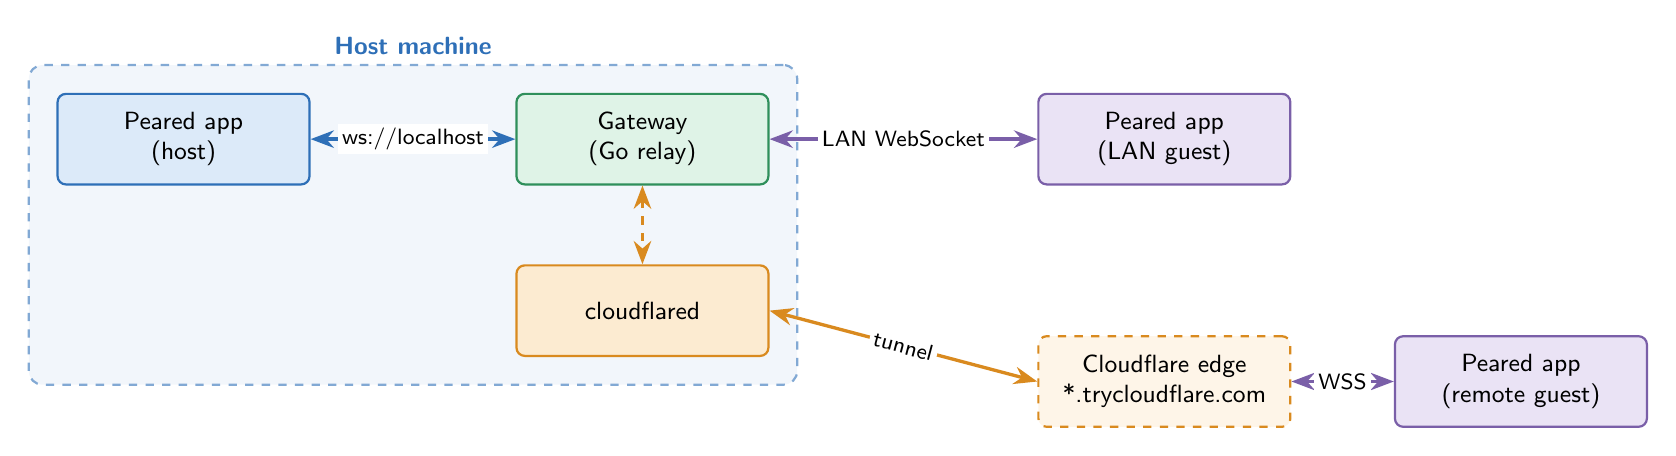
\begin{tikzpicture}[
      font=\small\sffamily,
      box/.style={draw, thick, rounded corners=3pt, align=center,
                  minimum width=3.2cm, minimum height=1.15cm},
      hostapp/.style={box, draw=pcblue, fill=pcblueL},
      side/.style={box, draw=pcgreen, fill=pcgreenL},
      tun/.style={box, draw=pcorange, fill=pcorangeL},
      guest/.style={box, draw=pcpurple, fill=pcpurpleL},
      cloud/.style={box, draw=pcorange, fill=pcorangeL!50, dashed},
      arr/.style={{Stealth}-{Stealth}, very thick, draw=black!70},
      lbl/.style={font=\footnotesize\sffamily, fill=white, inner sep=1.5pt}
    ]
    % host machine
    \node[hostapp] (app) {Peared app\\(host)};
    \node[side, right=2.6cm of app] (gw) {Gateway\\(Go relay)};
    \node[tun, below=1.0cm of gw] (cf) {cloudflared};

    % guests
    \node[guest, right=3.4cm of gw] (g1) {Peared app\\(LAN guest)};
    \node[cloud, below=1.9cm of g1] (edge) {Cloudflare edge\\ *.trycloudflare.com};
    \node[guest, right=1.3cm of edge] (g2) {Peared app\\(remote guest)};

    \begin{scope}[on background layer]
      \node[draw=pcblue!60, thick, dashed, rounded corners=5pt, fill=pcblue!6,
            inner sep=10pt, fit=(app)(gw)(cf),
            label={[font=\small\sffamily\bfseries, text=pcblue]above:Host machine}] {};
    \end{scope}

    \draw[arr, draw=pcblue] (app) -- node[lbl]{ws://localhost} (gw);
    \draw[arr, draw=pcpurple] (gw) -- node[lbl]{LAN WebSocket} (g1);
    \draw[arr, draw=pcorange] (cf.east) -- node[lbl, sloped]{tunnel} (edge.west);
    \draw[arr, draw=pcpurple] (edge) -- node[lbl]{WSS} (g2);
    \draw[arr, dashed, draw=pcorange] (gw) -- (cf);
  \end{tikzpicture}}
  \caption{სისტემის საერთო არქიტექტურა: ჰოსტის კომპიუტერზე გაშვებული
  გეითვეი და მასთან დაკავშირებული კლიენტები}
  \label{diag:architecture}
\end{diagram}

\paragraph{სესიის სასიცოცხლო ციკლი.}
როდესაც მომხმარებელი სესიას იწყებს (hosting), აპლიკაცია
თანმიმდევრულად ასრულებს შემდეგ ნაბიჯებს: (1) უშვებს გეითვეის პროცესს და
მისგან stdout-ზე დაბეჭდილი JSON შეტყობინებით იგებს,
რომელ პორტზე დაიწყო მუშაობა; (2) უშვებს
\texttt{cloudflared}-ს და ელოდება საჯარო ბმულს; (3) HTTP მოთხოვნით
გეითვეისგან ქმნის „ოთახს“ (room) და იღებს მის იდენტიფიკატორს; (4) თავად
უერთდება ოთახს WebSocket-ით და მაშინვე აგზავნის დოკუმენტის სნეფშოტს, რათა
მოგვიანებით შემოსული სტუმრები სწრაფად „დაეწიონ“ მიმდინარე მდგომარეობას.
ამის შემდეგ ჰოსტი ორ ბმულს იღებს,- ლოკალური ქსელის და საჯაროს.
სტუმრის მხარეს იგივე პროცესი ბევრად
მარტივია: ბმულის ჩასმა, WebSocket კავშირი, სნეფშოტის მიღება და მუშაობის
დაწყება.

სესიაში უფლებები ასიმეტრიულია: ჰოსტი ყოველთვის სრულუფლებიანია, ხოლო
სტუმრები, თუ ჰოსტმა არ მიუთითა, მხოლოდ კითხვის რეჟიმში ერთვებიან (ჰოსტს შეუძლია
სესიის დაწყებისას აირჩიოს, რომ სტუმრებს ჩაწერის უფლება ავტომატურად
მიეცეთ). სესიის მიმდინარეობისას ჰოსტი თითოეულ სტუმარს ინდივიდუალურად
ანიჭებს ან ართმევს ჩაწერის უფლებას, ამ მექანიზმის ტექნიკურ დეტალებს
ქვემოთ განვიხილავთ.

\subsubsection{Tauri ფრეიმვორკი კონცეპტუალურად}

desktop აპლიკაცია აგებულია Tauri 2 ფრეიმვორკზე \cite{tauri}. Tauri-ის
იდეა მარტივია: აპლიკაციის ინტერფეისი იწერება ჩვეულებრივი ვებ-ტექნოლოგიებით
(ჩვენს შემთხვევაში React + TypeScript) და ეშვება ოპერაციული სისტემის
ჩაშენებულ webview-ში, ხოლო „ნატიური“ ლოგიკა, ფაილებთან წვდომა, ქსელი,
პროცესების მართვა, იწერება Rust-ზე და ცალკე პროცესის ბირთვში ცხოვრობს.
ორ სამყაროს შორის კომუნიკაცია ხდება IPC-ით: ფრონტენდი იძახებს ბექენდის
„ბრძანებებს“ (commands), ბექენდი კი ფრონტენდს „ივენთებს“ (events) უგზავნის.
Electron-თან შედარებით Tauri-ის ბინარები გაცილებით მცირეა (ის Chromium-ს
არ აპაკეტებს) და ბექენდის ენად Rust გამოვიყენეთ.
CRDT ბიბლიოთეკა სწორედ Rust-ზეა დაწერილი და აპლიკაციაში პირდაპირ,
დანამატების გარეშე ჩაშენდა.

Tauri-ის კიდევ ერთი ფუნქცია, რომელსაც აქტიურად ვიყენებთ, არის
\emph{sidecar} ბინარები: გეითვეი და \texttt{cloudflared} აპლიკაციასთან
ერთად იდება და აპლიკაცია მათ სასიცოცხლო ციკლს სრულად აკონტროლებს -
მომხმარებელი ვერც კი ამჩნევს, რომ მის კომპიუტერზე ცალკე სერვერი გაეშვა.

\subsubsection{ფრონტენდი და Monaco, როგორც ბაზისი}

ინტერფეისის ბაზისად Monaco Editor \cite{monaco} ავირჩიეთ, იგივე
 კომპონენტი, რომელზეც VS Code-ია აშენებული. ეს არჩევანი ბევრ რამეს
გვაძლევს „უფასოდ“: სინტაქსის გაფერადება, მრავალკურსორიანი რედაქტირება,
undo/redo, ძებნა და keyboard shortcuts. ჩვენი ფრონტენდი
Monaco-ს გარშემოა აგებული: React მართავს აპლიკაციის შელს (გვერდითი
პანელი, სესიის სტატუსი, მონაწილეთა სია, ფაილების მენიუ), ხოლო Monaco -
თავად ტექსტს. ლოკალური ცვლილებები Monaco-დან ბექენდისკენ IPC ბრძანებებით
მიდის, remote მონაწილეების ცვლილებები კი ბექენდიდან ივენთებით ბრუნდება.

\begin{diagram}[htbp]
  \centering
  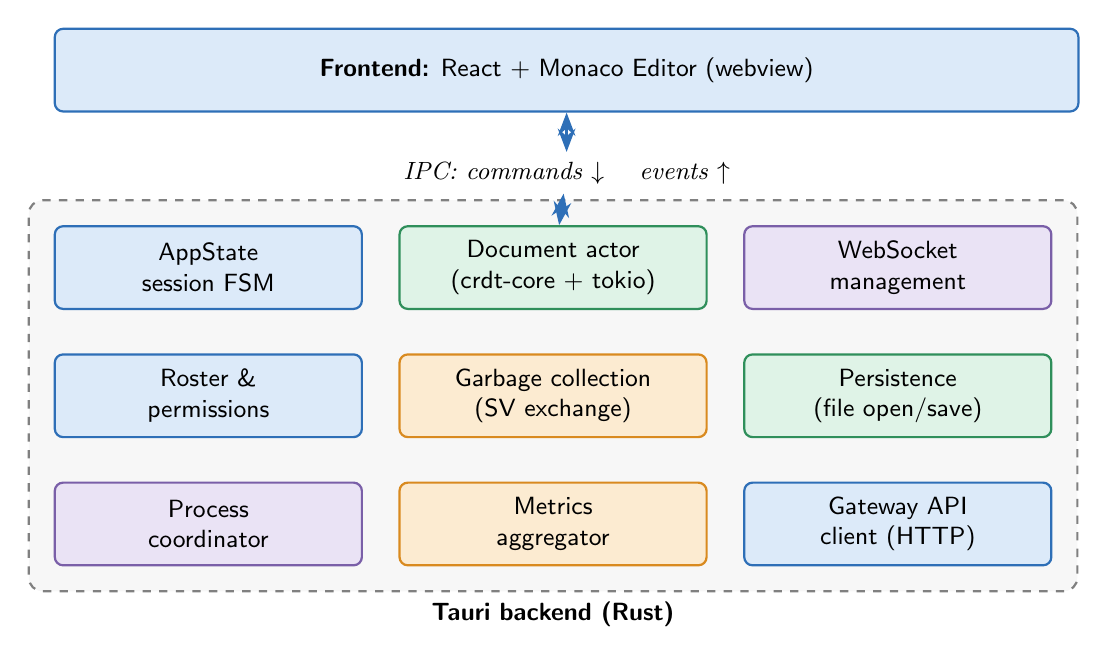
\begin{tikzpicture}[
      font=\small\sffamily,
      layer/.style={draw, thick, rounded corners=3pt, align=center,
                    minimum height=1.05cm, minimum width=3.9cm},
      arr/.style={{Stealth}-{Stealth}, very thick, draw=black!70}
    ]
    % Frontend
    \node[layer, draw=pcblue, fill=pcblueL, minimum width=13.0cm]
      (fe) {\textbf{Frontend:} React + Monaco Editor (webview)};
    \node[below=0.5cm of fe, font=\small\itshape] (ipc)
      {IPC: commands $\downarrow$ \quad events $\uparrow$};

    % Backend core row 1
    \node[layer, draw=pcblue, fill=pcblueL, below=0.4cm of ipc, xshift=-4.55cm]
      (appstate) {AppState\\session FSM};
    \node[layer, draw=pcgreen, fill=pcgreenL, right=0.45cm of appstate]
      (actor) {Document actor\\(crdt-core + tokio)};
    \node[layer, draw=pcpurple, fill=pcpurpleL, right=0.45cm of actor]
      (ws) {WebSocket\\management};

    % Backend row 2
    \node[layer, draw=pcblue, fill=pcblueL, below=0.55cm of appstate]
      (perm) {Roster \&\\permissions};
    \node[layer, draw=pcorange, fill=pcorangeL, right=0.45cm of perm]
      (gc) {Garbage collection\\(SV exchange)};
    \node[layer, draw=pcgreen, fill=pcgreenL, right=0.45cm of gc]
      (pers) {Persistence\\(file open/save)};

    % Backend row 3
    \node[layer, draw=pcpurple, fill=pcpurpleL, below=0.55cm of perm]
      (proc) {Process\\coordinator};
    \node[layer, draw=pcorange, fill=pcorangeL, right=0.45cm of proc]
      (metrics) {Metrics\\aggregator};
    \node[layer, draw=pcblue, fill=pcblueL, right=0.45cm of metrics]
      (gwapi) {Gateway API\\client (HTTP)};

    \begin{scope}[on background layer]
      \node[draw=black!50, thick, dashed, rounded corners=5pt, fill=black!3,
            inner sep=9pt, fit=(appstate)(ws)(proc)(gwapi),
            label={[font=\small\sffamily\bfseries]below:Tauri backend (Rust)}] {};
    \end{scope}

    \draw[arr, draw=pcblue] (fe) -- (ipc);
    \draw[arr, draw=pcblue] (ipc) -- (actor);
  \end{tikzpicture}
  \caption{კლიენტის (Tauri აპლიკაციის) შრეები და ქვესისტემები}
  \label{diag:layers}
\end{diagram}

\subsubsection{CRDT ბიბლიოთეკა (crdt-core)}

სისტემის მთავარი ნაწილია \texttt{crdt-core}, Rust-ზე დაწერილი დამოუკიდებელი
ბიბლიოთეკა, რომელიც YATA-ს სტილის ტექსტურ CRDT-ს მოიცავს. მისი პასუხისმგებლობაა დოკუმენტის
მდგომარეობა, ოპერაციების ინტეგრაცია და ბინარული (wire) ფორმატი.

\paragraph{ბლოკები და linked list.}
დოკუმენტი წარმოდგენილია \emph{ბლოკების} doubly linked list-ად. ბლოკი
არის ერთი ავტორის მიერ ზედიზედ აკრეფილი სიმბოლოების მონაკვეთი, რომელსაც
გააჩნია:
\begin{itemize}[itemsep=0pt]
  \item უნიკალური იდენტიფიკატორი \texttt{BlockId = (client\_id, clock)} -
        ავტორის ნომერი და მისი ლოკალური მთვლელი (ლამპორტის საათის
        ანალოგი).
        $n$ სიმბოლოიანი ბლოკი არის \texttt{(c, k)}-დან \texttt{(c, k+n-1)}-მდე;
  \item წარმოშობის ისტორია \texttt{origin\_left} და
        \texttt{origin\_right}, რომელი ორი ელემენტის შუაში დაიბადა ბლოკი
        ჩასმის მომენტში;
  \item შიგთავსი და წაშლის ბულეანი (\texttt{deleted}).
\end{itemize}

მთელი ტექსტის სიმბოლო-სიმბოლო შენახვის ნაცვლად ბლოკებით შენახვა
(მიდგომა, რომელიც Yjs-იდან გადმოვიღეთ \cite{yjs}) მეხსიერებასა და ქსელის
ტრაფიკს მკვეთრად ამცირებს: ჩვეულებრივი ბეჭდვისას მომდევნო სიმბოლო წინა
ბლოკს ეწებება/იმერჯება და ერთ ოპერაციად რჩება. ახალი ფაილის გახსნისას ტექსტი
64-სიმბოლოიან ბლოკებად იჭრება (\texttt{from\_text\_chunked}).

\paragraph{ბლოკის გაყოფა (splitting).}
რა ხდება, როდესაც ვინმე ბლოკის \emph{შუაში} ჩასვამს ტექსტს ან შუიდან
წაშლის? ბლოკი ორად იყოფა: მარცხენა ნახევარი ინარჩუნებს საწყის
იდენტიფიკატორს, მარჯვენა კი იღებს იმავე დიაპაზონის გაგრძელებას
(\texttt{(c, k+offset)}). რადგან იდენტიფიკატორები სინამდვილეში დიაპაზონებზეა
დამოკიდებული, ნებისმიერი
\texttt{BlockId} კვლავ ცალსახად პოულობს თავის ბლოკს, უბრალოდ ახლა შესაძლოა
ბლოკის შუაგულში აღმოჩნდეს. ეს ინვარიანტი (ე.წ. decomposition invariance)
კრიტიკულია: remote მონაწილის ოპერაცია შეიძლება ისეთ ბლოკზე განხორციელდეს,
რომელიც ჩვენთან უკვე სამ ნაწილად არის გაყოფილი.

\paragraph{ინტეგრაცია და კონფლიქტების გადაწყვეტა.}
remote ბლოკის მიღებისას ალგორითმმა უნდა იპოვოს მისი ზუსტი ადგილი
სიაში. თუ კონფლიქტი არ არის, ბლოკი უბრალოდ თავის origin-ებს შორის ჯდება.
თუ ორმა მონაწილემ ერთსა და იმავე ადგილას ერთდროულად ჩასვა ტექსტი
(ესეიგი თუ ორივე ბლოკს ერთი და იგივე origin-ები აქვს), YATA წესრიგს დეტერმინისტული
წესით ადგენს, კონფლიქტური ბლოკები ისე ლაგდება, რომ (1) ყველა რეპლიკაზე
ერთი და იგივე თანმიმდევრობა მიიღება და (2) ერთი ავტორის მიმდევრობითი
ჩანაწერები ერთად რჩება. Rust-ის type სისტემა აქ
ძალიან დაგვეხმარა: ინტეგრაციის ლოგიკა მკაცრად გამიჯნულ მოდულებშია
(\texttt{document/integrate.rs}) და ყოველი შემთხვევა ცალკე
ტესტითაა დაფარული.

\paragraph{წაშლა, DeleteSet და state ვექტორი.}
CRDT-ში წაშლა განსხვავებულად მუშაობს: ბლოკის ფიზიკურად ამოღება არ
შეიძლება, რადგან სხვა მონაწილის ჯერ მოუსვლელი ოპერაცია შესაძლოა სწორედ
მას ეყრდნობოდეს origin-ად. ამიტომ წაშლა მხოლოდ \emph{მონიშვნაა}: ბლოკი
რჩება სიაში როგორც tombstone, ტექსტში კი აღარ ჩანს.
წაშლები კომპაქტურად ინახება \texttt{DeleteSet} სტრუქტურაში, თითოეული
კლიენტისთვის წაშლილი \texttt{clock}-დიაპაზონების სიად.

\emph{state ვექტორი} ინახავს თითო კლიენტისთვის მისგან ნანახი ოპერაციების
მაქსიმალურ \texttt{clock}-ს. ორი რეპლიკის ვექტორების შედარებით ზუსტად ჩანს, რომელ
მხარეს აკლია რომელი ოპერაციები. ჩვენ ვექტორებს ორ რამეში ვიყენებთ:
გვიან შემოსული სტუმრის სინქრონიზაციასა და garbage collector-ში (იხ.
ოპტიმიზაციების თავი), სადაც ის განსაზღვრავს, რომელი წაშლა აქვს ყველას
გარანტირებულად ნანახი.

\paragraph{სნეფშოტები და wire პროტოკოლი.}
დოკუმენტის სრული მდგომარეობა, ბლოკები, DeleteSet, state ვექტორი -
სერიალიზდება \texttt{Snapshot} სტრუქტურად (ბინარულად, \texttt{bitcode}
ბიბლიოთეკით). ქსელში ყოველ ფრეიმს ერთბაიტიანი პრეფიქსი აქვს, რომელიც
ტიპს განსაზღვრავს: ოპერაცია (\texttt{0x00}), სნეფშოტი (\texttt{0x01}),
საკონტროლო ფრეიმი (\texttt{0x02}), garbage collector commit
(\texttt{0x04}), წევრობის ცვლილება (\texttt{0x05}), state ვექტორის
რეპორტი (\texttt{0x06}), უფლების ცვლილება (\texttt{0x07}) და მონაწილის
ინფორმაცია (\texttt{0x08}). რადგან ამ ფორმატს ორი ენა კითხულობს (Rust
კლიენტებში, Go გეითვეიში), ორივე მხარეს გვაქვს ე.წ. protocol drift
ტესტები.

\paragraph{პოზიციური B+ ინდექსი.}
CRDT ოპერაციები იდენტიფიკატორებზე მუშაობს, რედაქტორი კი, სიმბოლოს
პოზიციებზე („ჩასვი 42-ე პოზიციაზე“). ამ ორ სამყაროს შორის გადაყვანა
linked list-ის გავლით $O(n)$ ოპერაციაა და ყოველ კლავიშზე მთელი
დოკუმენტის ჩამოვლა დიდ ფაილებზე შესამჩნევად ანელებდა სისტემას. ამის
გადასაჭრელად დოკუმენტს დავურთეთ \emph{აუგმენტირებული B+ ხე}: ბლოკები ხის
ფოთლებში დოკუმენტის თანმიმდევრობისავით აწყვია, ხოლო ყოველი შიდა node
ინახავს შვილი ნოუდის (ქვე ხის) ხილული სიმბოლოების ჯამურ სიგრძეს (\texttt{visible\_len};
წაშლილი ბლოკის ხილული სიგრძე ნულია). პოზიციით ძებნისას ხეზე დაშვებისას
თითო დონეზე ვაკლებთ მარცხენა შვილების ჯამებს, $O(\log n)$; პირიქით,
ბლოკიდან პოზიციის გამოთვლისას ფოთლიდან ზემოთ ავდივართ და მარცხენა ძმების
ჯამებს ვაგროვებთ.

მნიშვნელოვანი დეტალი: ხე \emph{მეორეული, წარმოებული} სტრუქტურაა -
ჭეშმარიტების წყარო ყოველთვის doubly linked list რჩება. იმისთვის, რომ ისინი
არასდროს აცდნენ ერთმანეთს, debug რეჟიმში ყოველი მუტაციის შემდეგ ეშვება
ფუნქცია, რომელიც მთელ სიას ხელით ჩამოუვლის და ამოწმებს, რომ ხის პასუხები
ზუსტად ემთხვევა. 
ხის child node size განზრახ განსხვავებულია: debug-ში მცირეა (4),
რომ ტესტებში გაყოფის ლოგიკა ხშირად გავარჯიშდეს, release-ში კი დიდი რიცხვი ავიღეთ
(64/32), ნაკლები სიღრმე და უკეთესი კეშ-ლოკალურობა.

\begin{diagram}[htbp]
  \centering
  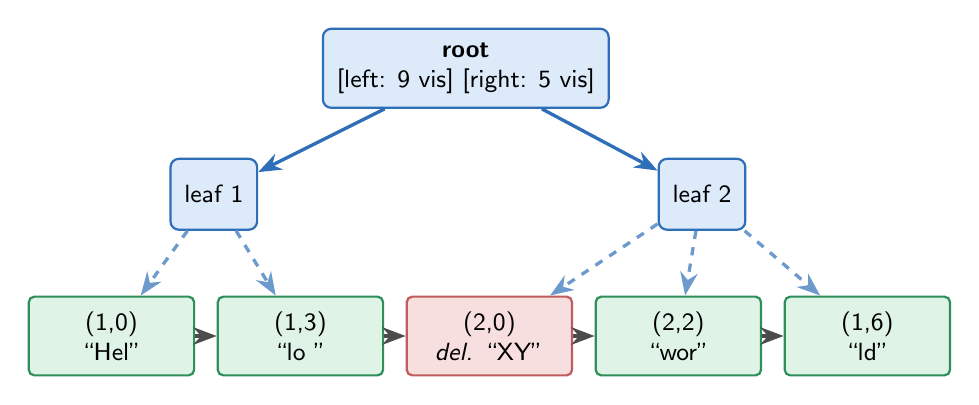
\begin{tikzpicture}[
      font=\small\sffamily,
      blk/.style={draw=pcgreen, thick, minimum height=1.0cm, minimum width=2.1cm,
                  align=center, fill=pcgreenL, rounded corners=2pt},
      tomb/.style={blk, draw=pcred, fill=pcredL},
      tnode/.style={draw=pcblue, thick, rounded corners=3pt, align=center,
                    fill=pcblueL, minimum height=0.9cm, inner sep=5pt},
      arr/.style={-{Stealth}, very thick, draw=black!70}
    ]
    % root
    \node[tnode] (root) at (4.5,3.4) {\textbf{root}\\{[}left: 9 vis{]} {[}right: 5 vis{]}};
    % leaves
    \node[tnode] (leafA) at (1.3,1.8) {leaf 1};
    \node[tnode] (leafB) at (7.5,1.8) {leaf 2};
    \draw[arr, draw=pcblue] (root) -- (leafA);
    \draw[arr, draw=pcblue] (root) -- (leafB);

    % linked list
    \node[blk]  (b1) at (0,0)   {(1,0)\\``Hel''};
    \node[blk]  (b2) at (2.4,0) {(1,3)\\``lo ''};
    \node[tomb] (b3) at (4.8,0) {(2,0)\\\emph{del.} ``XY''};
    \node[blk]  (b4) at (7.2,0) {(2,2)\\``wor''};
    \node[blk]  (b5) at (9.6,0) {(1,6)\\``ld''};
    \draw[arr] (b1) -- (b2);
    \draw[arr] (b2) -- (b3);
    \draw[arr] (b3) -- (b4);
    \draw[arr] (b4) -- (b5);

    \draw[arr, dashed, draw=pcblue!70] (leafA) -- (b1);
    \draw[arr, dashed, draw=pcblue!70] (leafA) -- (b2);
    \draw[arr, dashed, draw=pcblue!70] (leafB) -- (b3);
    \draw[arr, dashed, draw=pcblue!70] (leafB) -- (b4);
    \draw[arr, dashed, draw=pcblue!70] (leafB) -- (b5);
  \end{tikzpicture}
  \caption{CRDT დოკუმენტის სტრუქტურა: ბლოკების linked list
  (ქვემოთ, tombstone წითლადაა) და მასზე აგებული პოზიციური B+ ინდექსი
  (ზემოთ, კვანძებში, ხილული სიმბოლოების ჯამები)}
  \label{diag:crdt}
\end{diagram}

ჩასმისა და წაშლის დინამიკას ორი კადრ-კადრ დაშლილი დიაგრამა აჩვენებს
(დიაგრამები~\ref{diag:insert} და~\ref{diag:delete}): პირველი, თუ როგორ
ჯდება ახალი ბლოკი ერთდროულად სიაშიც და ხის ფოთოლშიც და როგორ „ბუბლდება“
ხილული სიგრძის დელტა ფესვამდე; მეორე, თუ როგორ იქცევა ბლოკი
tombstone-ად და როგორ სწორდება ჯამები მთელ შტოზე.

\begin{diagram}[htbp]
  \centering
  \begin{tikzpicture}[
      font=\footnotesize\sffamily,
      blk/.style={draw=pcgreen, thick, minimum height=0.85cm, minimum width=1.7cm,
                  align=center, fill=pcgreenL, rounded corners=2pt},
      newblk/.style={blk, draw=pcorange, fill=pcorangeL, very thick},
      tnode/.style={draw=pcblue, thick, rounded corners=3pt, align=center,
                    fill=pcblueL, minimum height=0.75cm, inner sep=4pt},
      hot/.style={draw=pcorange, very thick},
      arr/.style={-{Stealth}, thick, draw=black!70},
      steplbl/.style={anchor=west, font=\small\bfseries, text=pcblue}
    ]
    % ------------- Frame 1 -------------
    \begin{scope}[yshift=0cm]
      \node[steplbl] at (-0.9,3.0) {ნაბიჯი 1, საწყისი მდგომარეობა};
      \node[tnode] (r1) at (2.6,2.2) {root: [5 vis]};
      \node[tnode] (l1) at (2.6,1.1) {leaf: [(1,0):3] [(1,3):2]};
      \draw[arr, draw=pcblue] (r1) -- (l1);
      \node[blk] (a1) at (1.2,-0.1) {(1,0)\\``Hel''};
      \node[blk] (b1) at (4.0,-0.1) {(1,3)\\``lo''};
      \draw[arr] (a1) -- (b1);
    \end{scope}
    % ------------- Frame 2 -------------
    \begin{scope}[yshift=-4.3cm]
      \node[steplbl] at (-0.9,3.0) {ნაბიჯი 2, ახალი ბლოკი ჯდება სიაშიც და ფოთოლშიც};
      \node[tnode] (r2) at (2.6,2.2) {root: [5 vis]};
      \node[tnode, hot] (l2) at (2.6,1.1) {leaf: [(1,0):3] \textbf{[(2,0):2]} [(1,3):2]};
      \draw[arr, draw=pcblue] (r2) -- (l2);
      \node[blk] (a2) at (0.4,-0.1) {(1,0)\\``Hel''};
      \node[newblk] (n2) at (2.6,-0.1) {(2,0)\\``XY''};
      \node[blk] (b2) at (4.8,-0.1) {(1,3)\\``lo''};
      \draw[arr] (a2) -- (n2);
      \draw[arr] (n2) -- (b2);
    \end{scope}
    % ------------- Frame 3 -------------
    \begin{scope}[yshift=-8.6cm]
      \node[steplbl] at (-0.9,3.0) {ნაბიჯი 3, დელტა (+2) ბუბლდება ფესვამდე};
      \node[tnode, hot] (r3) at (2.6,2.2) {root: [\textbf{7} vis]};
      \node[tnode] (l3) at (2.6,1.1) {leaf: [(1,0):3] [(2,0):2] [(1,3):2]};
      \draw[arr, draw=pcblue] (r3) -- (l3);
      \draw[-{Stealth}, very thick, draw=pcorange]
        ($(l3.east)+(0.25,0)$) to[bend right=40]
        node[right, font=\small\sffamily\bfseries, text=pcorange]{+2} ($(r3.east)+(0.25,0)$);
      \node[blk] (a3) at (0.4,-0.1) {(1,0)\\``Hel''};
      \node[blk, draw=pcorange] (n3) at (2.6,-0.1) {(2,0)\\``XY''};
      \node[blk] (b3) at (4.8,-0.1) {(1,3)\\``lo''};
      \draw[arr] (a3) -- (n3);
      \draw[arr] (n3) -- (b3);
    \end{scope}
  \end{tikzpicture}
  \caption{ბლოკის ჩასმა ნაბიჯ-ნაბიჯ: ბლოკი ერთდროულად ემატება
  list-ს და ხის ფოთოლს, შემდეგ კი ხილული სიგრძის დელტა
  ფესვამდე ვრცელდება}
  \label{diag:insert}
\end{diagram}

\begin{diagram}[htbp]
  \centering
  \begin{tikzpicture}[
      font=\footnotesize\sffamily,
      blk/.style={draw=pcgreen, thick, minimum height=0.85cm, minimum width=1.7cm,
                  align=center, fill=pcgreenL, rounded corners=2pt},
      tomb/.style={blk, draw=pcred, fill=pcredL},
      tnode/.style={draw=pcblue, thick, rounded corners=3pt, align=center,
                    fill=pcblueL, minimum height=0.75cm, inner sep=4pt},
      hot/.style={draw=pcred, very thick},
      arr/.style={-{Stealth}, thick, draw=black!70},
      steplbl/.style={anchor=west, font=\small\bfseries, text=pcblue}
    ]
    % ------------- Frame 1 -------------
    \begin{scope}[yshift=0cm]
      \node[steplbl] at (-0.9,3.0) {ნაბიჯი 1, ბლოკი ინიშნება წაშლილად (tombstone)};
      \node[tnode] (r1) at (2.6,2.2) {root: [7 vis]};
      \node[tnode, hot] (l1) at (2.6,1.1) {leaf: [(1,0):3] \textbf{[(2,0):0]} [(1,3):2]};
      \draw[arr, draw=pcblue] (r1) -- (l1);
      \node[blk] (a1) at (0.4,-0.1) {(1,0)\\``Hel''};
      \node[tomb] (n1) at (2.6,-0.1) {(2,0)\\\emph{del.} ``XY''};
      \node[blk] (b1) at (4.8,-0.1) {(1,3)\\``lo''};
      \draw[arr] (a1) -- (n1);
      \draw[arr] (n1) -- (b1);
    \end{scope}
    % ------------- Frame 2 -------------
    \begin{scope}[yshift=-4.3cm]
      \node[steplbl] at (-0.9,3.0) {ნაბიჯი 2, დელტა ($-2$) ბუბლდება ფესვამდე};
      \node[tnode, hot] (r2) at (2.6,2.2) {root: [\textbf{5} vis]};
      \node[tnode] (l2) at (2.6,1.1) {leaf: [(1,0):3] [(2,0):0] [(1,3):2]};
      \draw[arr, draw=pcblue] (r2) -- (l2);
      \draw[-{Stealth}, very thick, draw=pcred]
        ($(l2.east)+(0.25,0)$) to[bend right=40]
        node[right, font=\small\sffamily\bfseries, text=pcred]{$-2$} ($(r2.east)+(0.25,0)$);
      \node[blk] (a2) at (0.4,-0.1) {(1,0)\\``Hel''};
      \node[tomb] (n2) at (2.6,-0.1) {(2,0)\\\emph{del.} ``XY''};
      \node[blk] (b2) at (4.8,-0.1) {(1,3)\\``lo''};
      \draw[arr] (a2) -- (n2);
      \draw[arr] (n2) -- (b2);
    \end{scope}
  \end{tikzpicture}
  \caption{ბლოკის წაშლა ნაბიჯ-ნაბიჯ: ბლოკი სიაში რჩება tombstone-ად,
  ხილული სიგრძე ნულდება და უარყოფითი დელტა ხის ჯამებს ასწორებს}
  \label{diag:delete}
\end{diagram}

\subsubsection{Tauri აპლიკაცია (desktop კლიენტი)}

Tauri აპლიკაციის Rust ბექენდი ის ადგილია, სადაც ყველა ქვესისტემა
ერთმანეთს ხვდება (იხ. დიაგრამა~\ref{diag:layers}): დოკუმენტის აქტორი,
WebSocket კავშირი, სესიის მდგომარეობის მანქანა, პროცესების მართვა, ნაგვის
შემგროვებელი, ფაილების შენახვა, უფლებების სისტემა და მეტრიკები.

\paragraph{დოკუმენტის აქტორი.}
ყველაზე მნიშვნელოვანი დიზაინის გადაწყვეტილება დოკუმენტთან წვდომის
ორგანიზებაა. გულუბრყვილო მიდგომა იქნებოდა \texttt{Mutex<Document>} -
საზიარო ობიექტი საკეტით, რომელსაც ყველა ნაკადი ეპოტინება. ამის ნაცვლად
\emph{აქტორის} ნიმუში გამოვიყენეთ: დოკუმენტს ფლობს ერთადერთი tokio
ამოცანა (\texttt{DocActor}), რომელიც უსასრულო ციკლში კითხულობს
შეტყობინებების არხს (\texttt{mpsc}). ნებისმიერი მოქმედება, ლოკალური
ჩასმა, დაშორებული ოპერაცია, სნეფშოტის აღება, ფაილში ჩასაწერი ტექსტის
წაკითხვა, არხში იგზავნება \texttt{DocOp} შეტყობინებად, პასუხი კი
ერთჯერადი (oneshot) არხით ბრუნდება. ამ მიდგომას რამდენიმე უპირატესობა
აქვს: საკეტები და deadlock-ის რისკი ქრება, ოპერაციები ბუნებრივად
სერიალიზდება (რაც CRDT-ისთვის ისედაც აუცილებელია), ხოლო ახალი ოპერაციის
დამატება მხოლოდ ახალი \texttt{DocOp} ვარიანტის და მისი დამმუშავებლის
დაწერას ნიშნავს. Rust-ის ownership სისტემა აქ ჩვენს სასარგებლოდ მუშაობს -
დოკუმენტზე მიმართვა აქტორის გარეთ უბრალოდ ვერ „გაიპარება“.

\paragraph{IPC, ბექენდიდან ფრონტენდამდე.}
როდესაც აქტორი დაშორებულ ცვლილებას აინტეგრირებს, ფრონტენდს Tauri ივენთს
უგზავნის: \texttt{crdt://remote-change} (პოზიცია და შიგთავსი),
\texttt{crdt://snapshot-applied} (დოკუმენტი მთლიანად შეიცვალა, მაგ.
სესიაში შესვლისას) ან \texttt{crdt://document-reset}. საპირისპირო
მიმართულებით ფრონტენდი \texttt{\#[tauri::command]} ბრძანებებს იძახებს:
\texttt{insert}, \texttt{delete}, \texttt{replace}, ფაილის ოპერაციები,
სესიის მართვა და ა.შ. საინტერესო ნიუანსი: webview-სა და ბექენდს შორის
შეტყობინებები ასინქრონულია, ამიტომ შესაძლებელია, რომ მომხმარებელმა
პოზიციაზე დააჭიროს მაშინ, როცა ბექენდში უკვე ჩამოვიდა (მაგრამ რედაქტორში
ჯერ არ ასახულა) სხვისი ცვლილება. ამის გამო ყოველი ლოკალური ბრძანება თან
ატარებს \texttt{base\_seq}-ს, ბოლო დაშორებული ცვლილების ნომერს, რომელიც
რედაქტორს ჰქონდა ნანახი ბრძანების გაგზავნისას. აქტორი ინახავს ბოლო
დაშორებული ოპერაციების მცირე ჟურნალს და შემოსული პოზიციის მათ მიმართ
ტრანსფორმაციას აკეთებს, პატარა, OT-ის სულისკვეთების ხიდი webview-სა და
ბექენდის რეპლიკას შორის, რომელმაც სინქრონიზაციის რთულად დასაჭერი ბაგები
აღმოფხვრა.

\paragraph{პროცესების მართვა.}
სესიის დაწყებისას \texttt{process\_coordinator} უშვებს გეითვეის sidecar-ს,
სტანდარტული გამოსავლიდან კითხულობს \texttt{\{"port": N\}} შეტყობინებას,
შემდეგ (საუკეთესო ძალისხმევით) უშვებს \texttt{cloudflared}-ს და ლოგებიდან
იჭერს გაცემულ საჯარო ბმულს. გეითვეისთან ავტორიზაციისთვის აპლიკაცია ყოველ
სესიაზე შემთხვევით bearer ტოკენს აგენერირებს და პროცესს გარემოს ცვლადით
გადასცემს, ამ ტოკენით ხდება ოთახის შექმნა და სესიის დასრულება (თავად
WebSocket შეერთება ტოკენს არ ითხოვს, რადგან სტუმრებს მისი ცოდნა არ
სჭირდებათ და არც უნდა სჭირდებოდეთ). ცალკე ყურადღება დაეთმო პროცესების
სიცოცხლის ციკლს: ფანჯრის დახურვისას აპლიკაცია სინქრონულად შლის ოთახს და
კლავს ორივე sidecar-ს, რომ მომხმარებელს „ობოლი“ სერვერი არ დარჩეს
ფონურად გაშვებული.

\paragraph{ასინქრონულობა და WebSocket მართვა.}
მთელი ბექენდი tokio-ს ასინქრონულ runtime-ზე დგას. WebSocket კავშირს სამი
დამოუკიდებელი tokio ამოცანა ემსახურება: \texttt{write\_loop} (გამავალი
ფრეიმების რიგი), \texttt{receive\_loop} (შემომავალი ბაიტების მიღება და
ტიპის ამოცნობა) და \texttt{process\_loop} (მიღებული ოპერაციების
გადაცემა დოკუმენტის აქტორისთვის და სხვა ქვესისტემებისთვის). ამოცანების ეს
გამიჯვნა ორ რამეს გვაძლევს: ნელი ქსელი ვერასდროს ბლოკავს დოკუმენტის
დამუშავებას, ხოლო კავშირის გაწყვეტისას საკმარისია სამივე ამოცანის
გაუქმება და მდგომარეობის გაწმენდა ერთ ადგილას (disconnect handler).

\paragraph{სესიის მდგომარეობის მანქანა.}
სესიის მდგომარეობა მკაცრი სასრული ავტომატია (FSM):
\texttt{Undecided} $\rightarrow$ \texttt{Starting} $\rightarrow$
\texttt{Host}/\texttt{Guest} $\rightarrow$ \texttt{Undecided}. ყველა
გადასვლა ვალიდირდება და უკანონო გადასვლა შეცდომას აბრუნებს. სესიის
წამოწყება მრავალსაფეხურიანი ასინქრონული პროცესია (პროცესების გაშვება,
ოთახის შექმნა, WebSocket კავშირი) და ნებისმიერ საფეხურზე შეიძლება
ჩავარდეს, ამიტომ \texttt{Starting} მდგომარეობას RAII „მცველი“ (guard)
იცავს: თუ ფუნქცია შეცდომით დასრულდა და მცველი ისე განადგურდა, რომ სესია
არ დასრულებულა, მდგომარეობა ავტომატურად ბრუნდება \texttt{Undecided}-ზე.
ასე გამოვრიცხეთ „გაჭედილი“ შუალედური მდგომარეობები ხელით rollback-ების
წერის გარეშე.

\paragraph{უფლებების მართვა.}
ჩაწერის უფლებების ავტორიტეტი გეითვეია: ის პირველ შემოერთებულს ჰოსტად
თვლის, ყოველ კლიენტს ჩაწერის დროშას უნახავს და წაკითხვის რეჟიმში მყოფი
კლიენტის ოპერაციებს უბრალოდ აგდებს (კლიენტის კოდის მოდიფიცირებული ვერსიაც
რომ შეეცადოს წესის გვერდის ავლას, გეითვეი მის ოპერაციებს არ გაავრცელებს).
ჰოსტი უფლების შეცვლას სპეციალური ფრეიმით (\texttt{0x07}) ითხოვს, გეითვეი
ამოწმებს, რომ მოთხოვნა ნამდვილად ჰოსტისგან მოდის, ცვლის დროშას და იმავე
ფრეიმს ყველას ავტორიტეტულ ექოდ უგზავნის. კლიენტის მხარეს
\texttt{roster} მოდული აწარმოებს მონაწილეთა სიას (სახელები, ჰოსტობა,
უფლებები), ხოლო სტუმრის საკუთარი უფლება \texttt{AppRole::Guest}-შივე
ინახება და \texttt{insert}/\texttt{delete}/\texttt{replace} ბრძანებებს
კარიბჭესავით კეტავს. ინტერფეისში ეს Monaco-ს \texttt{readOnly} რეჟიმად
აისახება. აქ ერთი ხრიკი დაგვჭირდა: Monaco წაკითხვის რეჟიმში პროგრამულ
ცვლილებებსაც ჩუმად აგდებს, ამიტომ დაშორებული ცვლილების ჩასმისას დროშას
წამიერად ვხსნით და ისევ ვაბრუნებთ.

\paragraph{ფაილების შენახვა და გახსნა.}
დოკუმენტი ორ ფორმატში ინახება, გაფართოების მიხედვით: ჩვეულებრივი ტექსტი
(ნებისმიერი გაფართოება) ან საკუთარი \texttt{.pcdoc} ფორმატი, \texttt{PCDC}
მაგიური ბაიტები, ვერსია და ბინარულად სერიალიზებული სრული CRDT სნეფშოტი,
ისტორიითა და იდენტიფიკატორებით. გახსნისას ფორმატს ვცნობთ არა
გაფართოებით, არამედ მაგიური ბაიტებით. ჩაწერა ყოველთვის ატომურია, ჯერ
დროებით ფაილში, შემდეგ გადარქმევით, რომ შენახვისას შეწყვეტამ (გათიშულმა
დენმა, ჩავარდნილმა პროცესმა) ნახევრად ჩაწერილი ფაილი არ დაგვიტოვოს.
ცალკე პრობლემა აღმოჩნდა ხაზის დაბოლოებები: Windows-ის ფაილები CRLF-ს
იყენებს, Monaco და CRDT კი LF-ს ელოდება. გახსნისას ტექსტს LF-ზე
ვანორმალიზებთ, ვიმახსოვრებთ, იყო თუ არა ფაილი CRLF-იანი, და შენახვისას
ისევ ვაბრუნებთ, ასე Windows-ის ფაილი ბაიტ-ბაიტ იდენტური ბრუნდება და
კროსპლატფორმულ სესიაშიც პოზიციები აღარ „ცურავს“ (ეს ბაგი რეალურად
გვქონდა და ქვემოთ, პრობლემების ნაწილში, ცალკე ვახსენებთ). ბოლოს,
აპლიკაცია ბოლო გახსნილი ფაილების სიას (MRU) აწარმოებს, სრულფასოვანი
ფაილ-მენეჯერის გარეშე, უბრალოდ სწრაფი წვდომისთვის.

\paragraph{მეტრიკების სისტემა.}
დიაგნოსტიკისთვის აპლიკაციას ჩაშენებული მეტრიკების პანელი აქვს. გეითვეი
ატომურ მთვლელებს აწარმოებს, აქტიური ოთახები და კლიენტები, გადაგზავნილი
ფრეიმების რაოდენობა და მოცულობა, სნეფშოტ-სინქრონიზაციების
წარმატება/ჩავარდნა, ნელი კლიენტების გათიშვები, და მათ HTTP ენდპოინტზე
აქვეყნებს. ჰოსტის აპლიკაციაში ცალკე tokio ამოცანა
(\texttt{process\_metrics\_aggregator}) პერიოდულად კითხულობს გეითვეის ამ
ენდპოინტს და \texttt{cloudflared}-ის საკუთარ მეტრიკებს, აერთიანებს მათ და
ივენთით ფრონტენდს აწვდის, სადაც მომხმარებელი მათ პანელში ხედავს. ეს
სესიის გამართვისას ძალიან გამოგვადგა, მაშინვე ჩანს, გადის თუ არა
ტრაფიკი და ვინ არის შეერთებული.

\subsubsection{ფრონტენდი}

ფრონტენდი React + TypeScript აპლიკაციაა (აწყობილი Vite-ით), რომლის
ცენტრშიც Monaco რედაქტორი დგას. მისი მთავარი ამოცანა ორმხრივი ნაკადის
გამართული მუშაობაა: ლოკალური keystrokes ბექენდისკენ, remote
ცვლილებები - რედაქტორისკენ.

\paragraph{ლოკალური ცვლილებების გაგზავნა.}
Monaco-ს ყოველი ცვლილება (\texttt{onDidChangeModelContent})
ითარგმნება IPC ბრძანებად: \texttt{insert}, \texttt{delete} ან
\texttt{replace}, პოზიციით და შიგთავსით. იმისთვის, რომ სწრაფი ბეჭდვისას
ბრძანებებმა ერთმანეთს არ გადაუსწრონ, ისინი ერთ ჯაჭვზე ეწყობა
(\texttt{opQueue}-ს მეშვეობით ყოველი შემდეგი ბრძანება წინას დასრულებას ელოდება).
თითო ბრძანებას თან მიჰყვება \texttt{baseSeq}, ბოლო remote ცვლილების
ნომერი, რომელიც რედაქტორს გაგზავნის მომენტში ჰქონდა ასახული, რომლითაც
ბექენდი პოზიციას გადათვლის როცა საჭიროა.

\paragraph{remote ცვლილებების მიღება.}
ბექენდის \texttt{crdt://remote-change} ივენთს ისმენს
\texttt{remoteChangeListener}, რომელიც ცვლილებას Monaco-ში პროგრამულად
ჩასვამს. აქ ორი ხაფანგი გვხვდება: ჯერ ერთი, პროგრამული ჩასმაც
\texttt{onDidChangeModelContent}-ს ააქტიურებს, რაც ცვლილებას უკან,
ბექენდისკენ გააბრუნებდა და უსასრულო ციკლს გააჩენდა, ამას ვკეტავთ
\texttt{isApplyingRemote} დროშით, რომელიც ჩასმის განმავლობაში ლოკალურ
დამმუშავებელს თიშავს. მეორე, წაკითხვის რეჟიმში მყოფ რედაქტორში Monaco
პროგრამულ ცვლილებებსაც უგულებელყოფს, ამიტომ remote ცვლილების ჩასმისას
\texttt{readOnly} დროშა წამიერად იხსნება. სნეფშოტის მიღებისას (მაგ.
სესიაში შესვლისას) ცალკე მსმენელი მთელ დოკუმენტს ანაცვლებს.

\paragraph{ინტერფეისის აგებულება.}
ვიზუალურად აპლიკაცია VS Code-ის სტილის გარსია: მარცხნივ ვიწრო 
side rail, რომელიც გვერდით პანელს ხსნის სამი სექციით -
ფაილები (გახსნა/შენახვა/ბოლო ფაილები), თანამშრომლობა (სესიის
წამოწყება/შეერთება/დატოვება) და პერსონალური პარამეტრები (სახელი, თემა,
ფონტის ზომა). ზედა ზოლში სესიის სტატუსი, მონაწილეთა ავატარები
(თითოეულს დეტერმინისტულად გამოთვლილი ფერი აქვს), მოსაწვევი ბმულების
popover და მენიუა. ინტერფეისის მდგომარეობა React ჰუკებშია
ორგანიზებული (\texttt{useRoomState}, \texttt{useSessionEvents},
\texttt{useWritePermission}, \texttt{useTheme} და ა.შ.), რომლებიც
ბექენდის ივენთებს უსმენენ და კომპონენტებს უბრალო props-ებით კვებავენ.

ფრონტენდის ვიზუალური დიზაინის იტერაციებში (ფერთა პალიტრა, კომპონენტების
განლაგება, თემები) დამხმარე ინსტრუმენტად ვიყენებდით Claude-ს
\cite{claude}; საბოლოო დიზაინის გადაწყვეტილებები და მათი იმპლემენტაცია
გუნდის წევრებისაა.

ფრონტენდს აქვს საკუთარი ტესტებიც (vitest): სინქრონიზაციის კრიტიკული
დამხმარე ლოგიკა, შებრუნებული რედაქტირებების გამოთვლა და
\texttt{baseSeq}-ის აღრიცხვა, ავტომატურად მოწმდება, ხოლო ტიპიზაცია და
ლინტერი CI-ში ეშვება.

\subsubsection{Gateway (Go relay სერვერი)}

Gateway dumb relay ტიპის სერვერია: ის დოკუმენტის შესახებ
არაფერს ინახავს, არც სნეფშოტს, არც ოპერაციების ისტორიას არც CRDT
დოკუმენტს. მისი საქმეა ოპერაციების კლიენტებთან სწრაფად გადაგზავნა. 

მისი ძირითადი ცნებებია:
\begin{itemize}[itemsep=0pt]
  \item \textbf{Hub}, ოთახების რეესტრი: ქმნის ოთახებს (\texttt{POST
        /rooms}), პოულობს მათ იდენტიფიკატორით და შლის სესიის ბოლოს;
  \item \textbf{Room}, ერთი სესიის სივრცე: წევრების სია და გადაგზავნის
        ლოგიკა. მიღებული ფრეიმი ეგზავნება ოთახის ყველა წევრს გამგზავნის
        გარდა;
  \item \textbf{Client}, Room-ის წევრი კლიენტის სტრუქტურა. 
\end{itemize}

მიუხედავად dumb როლისა, გეითვეი სერვერს რამდენიმე აქტიური მოვალეობა მაინც
აქვს. ახალი წევრის შემოსვლისას ის ჰოსტს სნეფშოტის მოთხოვნის საკონტროლო
ფრეიმს უგზავნის და ჰოსტის პასუხს მხოლოდ ახალ წევრს გადასცემს, ასე
გვიან შემოსული სტუმარი სწრაფად იღებს დოკუმენტის მიმდინარე მდგომარეობას,
ისე, რომ სერვერს დოკუმენტის შენახვა არ სჭირდება. წევრის ყოველ
შემოსვლა-გასვლაზე ოთახი ყველა Peer-ს ატყობინებს და ახალ წევრს, არსებული წევრებზე სრულ ინფორმაციას გადასცემს.
გეითვეი ასევე ინახავს Permission data-ს კლიენტებზე და კლიენტებისგან შემოსული data-ზე ახდენს შესაბამის ვალიდაციებს:
არ აკეთებს ისეთი ფრეიმების დაგზავნას, რომლის გამომგზავნსაც write პრივილეგია არ აქვს.

უსაფრთხოებისა და მდგრადობის მხრივ: ყველა HTTP ენდპოინტი (გარდა
\texttt{/health} და \texttt{/ws}) მოითხოვს bearer ტოკენს, რომელიც მხოლოდ
ჰოსტის აპლიკაციამ იცის; HTTP endpoint-ები დაცულია IP Rate Limiter-ით. 

\subsubsection{სისტემის ოპტიმიზაცია}

პროექტის მეორე ნახევარში ორი დიდი ოპტიმიზაცია განვახორციელეთ: პოზიციური
B+ ინდექსი და ნაგვის შემგროვებელი სისტემა. ორივე იმ პრობლემებს პასუხობს,
რომლებიც ყველა სერიოზულ CRDT იმპლემენტაციას აწუხებს და რომელთა
გადაწყვეტასაც Yjs \cite{yjs} საკუთარ დიზაინში დიდ ადგილს უთმობს.

\paragraph{პოზიციური B+ ინდექსი რიცხვებში.}
ინდექსის აგებულება CRDT-ის თავში აღვწერეთ; აქ მის ეფექტზე ვისაუბრებთ.
ოპტიმიზაციამდე ყოველი კლავიში დოკუმენტის დაკავშირებული სიის თავიდან
ჩამოვლას მოითხოვდა, $O(n)$ ორივე მიმართულებით (პოზიციიდან ბლოკამდე და
ბლოკიდან პოზიციამდე). მცირე ფაილებზე ეს შეუმჩნეველია, მაგრამ ბლოკების
რაოდენობის ზრდასთან ერთად ღირებულება წრფივად იზრდება და ეს ღირებულება
\emph{ყოველ} კლავიშზე და \emph{ყოველ} დაშორებულ ოპერაციაზე გადაიხდება.
ჩვენი გაზომვებით (debug ბილდი, სადაც ხის განშტოების ფაქტორი განზრახ
მცირეა):

\begin{table}[htbp]
  \centering
  \begin{tabular}{rrrr}
    \toprule
    ბლოკების რაოდენობა & სიის ჩამოვლა ($O(n)$) & B+ ხე ($O(\log n)$) & აჩქარება \\
    \midrule
    $\sim$200    & $\sim$127~$\mu$s  & $\sim$14~$\mu$s & $9\times$ \\
    1\,000       & $\sim$620~$\mu$s  & $\sim$16~$\mu$s & $\sim 39\times$ \\
    10\,000      & $\sim$6\,200~$\mu$s & $\sim$18~$\mu$s & $\sim 340\times$ \\
    \bottomrule
  \end{tabular}
  \caption{პოზიციის ძებნის დრო ინდექსამდე და ინდექსის შემდეგ}
  \label{tab:btree}
\end{table}

საკვანძო დაკვირვება ისაა, რომ ხის სვეტი თითქმის მუდმივია, ლოგარითმი
პრაქტიკაში „ბრტყელია“. Release ბილდში (განშტოება 64/32, სრული
ოპტიმიზაციები) თითო ძებნა 1~$\mu$s-ზე ნაკლებია დოკუმენტის ზომის მიუხედავად,
ანუ რედაქტორის კადრის ბიუჯეტს ინდექსი ვერასდროს ემუქრება. ეს ზუსტად ის
მიზეზია, რის გამოც მოწიფული CRDT იმპლემენტაციები (Yjs, diamond-types
\cite{diamond}) მსგავს ინდექსებს აუცილებლობად თვლიან.

\paragraph{ნაგვის შემგროვებელი, რატომ არის საჭირო.}
როგორც აღვნიშნეთ, CRDT-ში წაშლა მხოლოდ მონიშვნაა და წაშლილი ბლოკები
tombstone-ებად რჩება. აქტიური რედაქტირებისას ეს სწრაფად გროვდება:
დიდხანს მიმდინარე სესიაში დოკუმენტის მეხსიერების უმეტესი ნაწილი შესაძლოა
დიდი ხნის წაშლილმა ტექსტმა დაიკავოს, რომელიც სნეფშოტებთან ერთად
ქსელშიც მოგზაურობს. tombstone-ის უბრალოდ წაშლა კი საშიშია: თუ რომელიმე
მონაწილემ ის ჯერ არ ნახა, ან თუ დაგვიანებული ოპერაცია მას origin-ად
ეყრდნობა, ნაადრევი წაშლა რეპლიკების უხმო დაშორებას (divergence)
გამოიწვევს. სწორედ ამიტომ ეთმობა Yjs-ში ნაგვის შეგროვებას ცალკე,
საკმაოდ ფაქიზი მექანიზმი.

\paragraph{ჩვენი მიდგომის თავისებურება.}
აქ ვისარგებლეთ ჩვენი არქიტექტურის ერთი თვისებით, რომელიც „სუფთა“
peer-to-peer სისტემებს არ აქვთ: ჩვენს სესიას ჰყავს გამორჩეული კვანძი -
ჰოსტი, რომელიც ყოველთვის ონლაინაა (სესია მის გარეშე ვერ არსებობს) და
რომელსაც გეითვეი წევრობის ზუსტ სურათს აწვდის. ეს ჰოსტს ბუნებრივ
კოორდინატორად აქცევს, ისე, რომ დოკუმენტის მონაცემები მაინც სრულად
დეცენტრალიზებული რჩება. სქემა ასე მუშაობს:

\begin{enumerate}[itemsep=0pt]
  \item ყოველი სტუმარი პერიოდულად (დებაუნსით, რომ ქსელი არ გადაიტვირთოს)
        აქვეყნებს თავის მდგომარეობის ვექტორს, „აი, რამდენი მაქვს
        ნანახი თითოეული ავტორისგან“;
  \item ჰოსტი აგროვებს ყველა წევრის ვექტორს (გეითვეის წევრობის ფრეიმები
        ეუბნება, ვინ არის ამჟამად ოთახში) და ითვლის მათ \emph{მინიმუმს} -
        „იატაკს“: ოპერაციების იმ ზღვარს, რომელიც ყველას გარანტირებულად
        აქვს ნანახი;
  \item ამ იატაკს ჰოსტი კვეთს საკუთარ DeleteSet-თან და იღებს
        „დადასტურებული“ წაშლების სიმრავლეს, წაშლებს, რომლებიც ყველამ
        ნახა;
  \item დადასტურებული დიაპაზონები \texttt{gc-commit} ფრეიმად ეგზავნება
        ყველა მონაწილეს (და ჰოსტისვე დოკუმენტს), რომლებიც მას
        ერთნაირად ასრულებენ.
\end{enumerate}

\texttt{gc-commit}-ის შესრულება განზრახ კონსერვატიულია: ბლოკები
სტრუქტურულად \emph{არ} იშლება, მხოლოდ მათი ტექსტური შიგთავსი იცლება და
სნეფშოტისთვის განკუთვნილი წაშლის სიმრავლეები იკვეცება. ბლოკის
იდენტიფიკატორი და ადგილი სიაში უცვლელი რჩება, ამიტომ დაგვიანებული
ოპერაცია, რომელიც ამ ბლოკს origin-ად იყენებს, ისევ ზუსტად ინტეგრირდება -
სწორედ ეს ხდის ჩვენს ნაგვის შეგროვებას კონვერგენციისთვის უსაფრთხოს.
სტრუქტურული წაშლა შემდეგი ნაბიჯი იქნებოდა, მაგრამ ის ინტეგრაციის
ალგორითმის ინვარიანტებს არღვევს (გაყოფის მიმართ ინვარიანტულობა დაიკარგება)
და მეხსიერების მოგება რისკად არ ღირს, მთავარი მოგება (ტექსტის
გათავისუფლება და სნეფშოტების შემცირება) ისედაც მიიღწევა.

რამდენადაც ჩვენთვის ცნობილია, ეს ჰოსტ-ავტორიტეტული,
მდგომარეობის-ვექტორის-იატაკზე დაფუძნებული სქემა განსხვავდება გავრცელებული
CRDT იმპლემენტაციების მიდგომებისგან, რომლებიც ან სრულად სიმეტრიულ
პროტოკოლებს იყენებენ, ან ნაგვის შეგროვებას საერთოდ დოკუმენტის „შენახვის“
მომენტამდე დებენ. ჩვენს შემთხვევაში ჰოსტის გამორჩეულობა ისედაც სისტემის
ნაწილი იყო, მისი გამოყენება ნაგვის შეგროვების გასამარტივებლად
არქიტექტურის ბუნებრივი გაგრძელება აღმოჩნდა.

\paragraph{პრობლემები, რომლებსაც გზაში გადავაწყდით.}
გაიდლაინის შესაბამისად, აქვე შევაჯამებთ განვითარებისას წამოჭრილ
მნიშვნელოვან პრობლემებსა და მათ გადაწყვეტებს:

\begin{itemize}[itemsep=2pt]
  \item \textbf{პოზიციების „ცურვა“ webview-სა და ბექენდს შორის} -
        ასინქრონული IPC-ის გამო ლოკალური ბრძანება შესაძლოა მოძველებულ
        პოზიციას ატარებდეს. გადაწყვეტა: \texttt{baseSeq} +
        ბექენდში დაშორებული ოპერაციების მცირე ჟურნალის მიმართ პოზიციის
        ტრანსფორმაცია.
  \item \textbf{Windows-ის CRLF დესინქრონიზაცია}, CRLF-იანი ფაილის
        გახსნისას პოზიციები პლატფორმებს შორის აღარ ემთხვეოდა და
        ხაზის შუაში რედაქტირება ცდებოდა. გადაწყვეტა: LF-ზე ნორმალიზაცია
        გახსნისას და CRLF-ის აღდგენა შენახვისას.
  \item \textbf{Monaco-ს readOnly ხაფანგი}, წაკითხვის რეჟიმში Monaco
        პროგრამულ რედაქტირებებსაც აგდებდა და სტუმარი დაშორებულ
        ცვლილებებს ვეღარ იღებდა. გადაწყვეტა: დროშის წამიერი მოხსნა
        დაშორებული ცვლილების ჩასმისას.
  \item \textbf{სნეფშოტ-სინქრონიზაციის რბოლა}, თავდაპირველად ჰოსტი
        სნეფშოტს მხოლოდ შეერთებისას აგზავნიდა და გვიან შემოსული სტუმარი
        შესაძლოა მოძველებულ მდგომარეობას იღებდა. გადაწყვეტა: მოთხოვნა-
        პასუხის სქემა, გეითვეი ყოველ ახალ წევრზე ჰოსტს \emph{ახალ}
        სნეფშოტს სთხოვს.
  \item \textbf{დიდი ჩასმების დანაწევრება}, გიგანტური ერთიანი ბლოკები
        (მაგ. მთელი ფაილის ჩასმა) ინდექსსა და ქსელს ტვირთავდა.
        გადაწყვეტა: ტექსტის 64-სიმბოლოიან ბლოკებად დაჭრა გახსნისას.
  \item \textbf{ინდექსისა და სიის დაშორება}, B+ ხის დანერგვისას
        ყველაზე სახიფათო რისკი ორი სტრუქტურის უხმო დაშორება იყო.
        გადაწყვეტა: debug-ორაკული, რომელიც ყოველი მუტაციის შემდეგ სრულ
        შედარებას აკეთებს, პლუს ხის შიდა ინვარიანტების ცალკე ვალიდატორი.
\end{itemize}

\subsection{მიღებული შედეგი და შეფასება}

პროექტის საბოლოო შედეგი არის მომუშავე, კროსპლატფორმული desktop
აპლიკაცია, რომელიც Linux-ზე, Windows-სა და macOS-ზე ეშვება. ტიპური
workflow ასე გამოიყურება: პირველი გაშვებისას მომხმარებელი სახელს
ირჩევს (იმახსოვრება შემდეგი გაშვებებისთვის), შემდეგ ხსნის ან ქმნის
დოკუმენტს და გვერდითი პანელიდან იწყებს სესიას (ფაილების სექცია, იხ.
სურათი~\ref{fig:files}). აპლიკაცია რამდენიმე წამში
აბრუნებს ორ მოსაწვევ ბმულს, ლოკალური ქსელისა და საჯაროს (იხ.
სურათი~\ref{fig:host}). სტუმრები საკუთარ აპლიკაციაში ბმულს ჩასვამენ
და მაშინვე ხედავენ დოკუმენტის მიმდინარე მდგომარეობას; ყველა შემდგომი
ცვლილება ყველასთან რეალურ დროში აისახება. ჰოსტი peers პანელიდან
მართავს, ვის შეუძლია რედაქტირება (იხ. სურათი~\ref{fig:guest}), ხოლო
ნამუშევარი ნებისმიერ დროს ინახება როგორც ჩვეულებრივ ტექსტურ ფაილად, ისე
\texttt{.pcdoc} ფორმატში (სრული ისტორიით). სესიის მდგომარეობის
სადიაგნოსტიკოდ ჩაშენებულია მეტრიკების პანელი (იხ.
სურათი~\ref{fig:metrics}).

\appscreenshot{images/1.png}{ფაილების სექცია: შენახვა, გახსნა, Fork და
ბოლო ფაილების სია}{fig:files}

\appscreenshot{images/2.png}{ჰოსტის ხედი: gateway/tunnel სტატუსი,
მოსაწვევი ბმულები და Invite ღილაკი (statusline-ზე ჩანს HOST როლი და
room id)}{fig:host}

\appscreenshot{images/3.png}{სტუმრის ხედი read-only რეჟიმში და peers
პანელი, სადაც ჩანს ჰოსტი და read-only სტუმარი}{fig:guest}

\appscreenshot{images/4.png}{მეტრიკების პანელი: გეითვეის live
სტატისტიკა (კლიენტები, ოთახები, გადაგზავნილი ფრეიმები, uptime)}{fig:metrics}

\paragraph{მიზნების შესრულება.}
შესავალში ჩამოყალიბებული ოთხივე მიზანი მიღწეულია: (1) სესიის დაწყება და
ბმულით შეერთება მუშაობს ორივე ქსელურ რეჟიმში, ლოკალურ ქსელში
ინტერნეტის გარეშე და გლობალურად Cloudflare Tunnel-ით; (2) პარალელური
რედაქტირება უკონფლიქტოდ ერწყმის YATA CRDT-ით და მონაწილეები
გარანტირებულად ერთსა და იმავე ტექსტს ხედავენ; (3) ინფრასტრუქტურის მართვა
სრულად ავტომატიზებულია, მომხმარებელი სერვერს ვერც ამჩნევს; (4) ჰოსტი
სესიას სრულად აკონტროლებს უფლებების ინდივიდუალური მართვით.

\paragraph{ხარისხის უზრუნველყოფა.}
სამივე კომპონენტს საკუთარი ტესტები აქვს: CRDT ბიბლიოთეკაში
ინტეგრაციის, splitting-ის, წაშლისა და ინდექსის ტესტები (მათ შორის
კონფლიქტური სცენარები), გეითვეიში ოთახის, გადაგზავნისა და permission
ტესტები, ფრონტენდზე სინქრონიზაციის ლოგიკის ტესტები. ბინარულ პროტოკოლს
ორივე მხარეს protocol drift ტესტები იცავს. CI (GitHub Actions) ყოველ
ცვლილებაზე უშვებს ფორმატირების, ლინტერების, ტესტებისა და უსაფრთხოების
შემოწმებებს (\texttt{cargo audit}, \texttt{npm audit},
\texttt{govulncheck}).

\paragraph{დარჩენილი შეზღუდვები.}
აღსანიშნავია ისიც, რაც სისტემას ჯერ არ შეუძლია: სესია ერთ დოკუმენტზეა
შემოსაზღვრული (მრავალფაილიანი პროექტების მხარდაჭერა არ არის), მონაწილეთა
კურსორები ერთმანეთისთვის ჯერ არ ჩანს, ხოლო ჰოსტის გათიშვა სესიას
ასრულებს. ეს პუნქტები სამომავლო განვითარების ბუნებრივი კანდიდატებია
(იხ. დასკვნა).


\clearpage
\section{დასკვნა}

Peared-ის შექმნამ ერთ პროექტში მოაქცია ის, რასაც ჩვეულებრივ რამდენიმე
სხვადასხვა კურსი ფარავს: დისტრიბუციული სისტემები (CRDT,
State Vector Exchange სისტემა, Garbage collection სისტემა), მონაცემთა სტრუქტურები
(აუგმენტირებული B+ ხე), სისტემური პროგრამირება Rust-ზე, ქსელური
პროგრამირება Go-ზე და თანამედროვე დესკტოპ/ვებ ინტერფეისები. საბოლოო
პროდუქტი, ერთობლივი რედაქტორი, რომელიც ცენტრალური სერვისის გარეშე
მუშაობს როგორც ლოკალურ, ისე გლობალურ ქსელში, თავიდანვე დასახულ მიზანს
პასუხობს და რეალურ სცენარში (აუდიტორია არასტაბილური ინტერნეტით) ნამდვილად
გამოსადეგია.

ტექნიკური ცოდნის მიღმა პროექტმა რამდენიმე უფრო ზოგადი გაკვეთილი
გვასწავლა. პირველი, კორექტულობის ინფრასტრუქტურის ღირებულება: debug-
ორაკულმა, protocol drift ტესტებმა და მკაცრმა CI-მ განაწილებული სისტემის
ყველაზე საშიში კლასის შეცდომები (რეპლიკების უხმო დაშორება) განვითარების
ეტაპზევე დაიჭირა, სანამ ისინი „იშვიათ, გაუმეორებელ ბაგებად“ იქცეოდნენ.
მეორე, აბსტრაქციის საზღვრების სწორად გავლება: ის, რომ \texttt{crdt-core}
არაფერს იცის ქსელზე, გეითვეი არაფერს იცის დოკუმენტზე, ხოლო ფრონტენდი
არაფერს იცის CRDT-ზე, სამივე კომპონენტის დამოუკიდებლად ტესტირებას და
პარალელურად განვითარებას აძლევდა საშუალებას. მესამე, გუნდური მუშაობის დისციპლინა: სამი ადამიანის
ნამუშევრის ყოველდღიური შერწყმა pull request-ებით, კოდის განხილვით და
ავტომატური შემოწმებებით თავად პროექტის ისეთივე ნაწილი აღმოჩნდა, როგორც
ალგორითმები.


% ============================================================
% ლიტერატურა (IEEE სტილი, ხელით)
% ============================================================
\clearpage
\addcontentsline{toc}{section}{გამოყენებული ლიტერატურა}
\begin{thebibliography}{9}

\bibitem{yata}
P.~Nicolaescu, K.~Jahns, M.~Derntl, and R.~Klamma,
``Near Real-Time Peer-to-Peer Shared Editing on Extensible Data Types,''
in \emph{Proceedings of the 19th International Conference on Supporting Group Work (GROUP~'16)},
Sanibel Island, FL, USA, 2016, pp. 39--49.

\bibitem{crdt}
M.~Shapiro, N.~Preguiça, C.~Baquero, and M.~Zawirski,
``Conflict-free Replicated Data Types,''
in \emph{Proceedings of the 13th International Symposium on Stabilization, Safety, and Security of Distributed Systems (SSS~'11)},
Grenoble, France, 2011, pp. 386--400.

\bibitem{ot}
C.~A. Ellis and S.~J. Gibbs,
``Concurrency control in groupware systems,''
in \emph{Proceedings of the 1989 ACM SIGMOD International Conference on Management of Data},
Portland, OR, USA, 1989, pp. 399--407.

\bibitem{yjs}
K.~Jahns, ``Yjs Documentation.'' [Online]. Available: \url{https://docs.yjs.dev/}

\bibitem{diamond}
J.~Gentle, ``diamond-types: The world's fastest CRDT.'' [Online]. Available: \url{https://github.com/josephg/diamond-types}

\bibitem{tauri}
Tauri Working Group, ``Tauri 2.0 Documentation.'' [Online]. Available: \url{https://v2.tauri.app/}

\bibitem{monaco}
Microsoft, ``Monaco Editor.'' [Online]. Available: \url{https://microsoft.github.io/monaco-editor/}

\bibitem{cloudflared}
Cloudflare, Inc., ``Cloudflare Tunnel Documentation.'' [Online]. Available: \url{https://developers.cloudflare.com/cloudflare-one/connections/connect-networks/}

\bibitem{claude}
Anthropic, ``Claude.'' [Online]. Available: \url{https://claude.com/}
(გამოყენებულია ფრონტენდის ვიზუალური დიზაინის იტერაციებში დამხმარე ინსტრუმენტად)

\end{thebibliography}

% ============================================================
% დანართები
% ============================================================
\clearpage
\section{დანართები}
\begin{itemize}
  \item პროექტის GitHub ბმული: \url{https://github.com/CarlTeapot/Peared}
\end{itemize}

\end{document}
